\documentclass[a4paper,11pt,exos]{nsi} % COMPILE WITH DRAFT


%\pagestyle{empty}
\begin{document}



\classe{\premiere spe}
\titre{Exercices Probabilités conditionnelles}
\maketitle

\subsection*{Probabilités}

\exo{ Représenter des événements}
	Représenter chacun des événements suivants sur le diagramme de Venn :
	\begin{multicols}{3}
		\begin{enumerate}
			\item 	$A\cap B$
			\begin{center}
				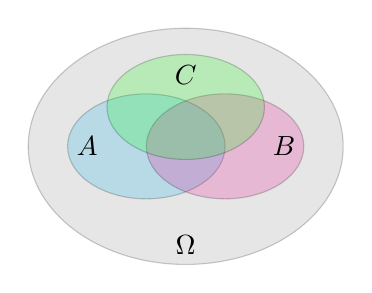
\begin{tikzpicture}[scale = 4/8]
					\draw[fill = gray, opacity=.2] (1,0) ellipse (4 and 3);
					\draw[fill = cyan,opacity = .2](0,0) ellipse (2 and 4/3);
					\draw[fill = magenta,opacity = .2](2,0) ellipse (2 and 4/3);
					\draw[fill = green,opacity = .2](1,1) ellipse (2 and 4/3);
					\draw (-1.5,0) node{$A$};
					\draw (3.5,0) node{$B$};
					\draw (1,1.8) node{$C$};
					\draw(1,-2.5) node {$\Omega$};
				\end{tikzpicture}
			\end{center}
			\item 	$A\cup C$
			\begin{center}
				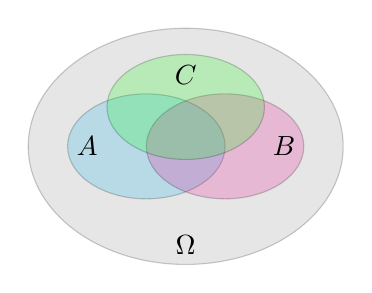
\begin{tikzpicture}[scale = 4/8]
					\draw[fill = gray, opacity=.2] (1,0) ellipse (4 and 3);
					\draw[fill = cyan,opacity = .2](0,0) ellipse (2 and 4/3);
					\draw[fill = magenta,opacity = .2](2,0) ellipse (2 and 4/3);
					\draw[fill = green,opacity = .2](1,1) ellipse (2 and 4/3);
					\draw (-1.5,0) node{$A$};
					\draw (3.5,0) node{$B$};
					\draw (1,1.8) node{$C$};
					\draw(1,-2.5) node {$\Omega$};
				\end{tikzpicture}
			\end{center}
			\item 	$\overline{A}$
			\begin{center}
				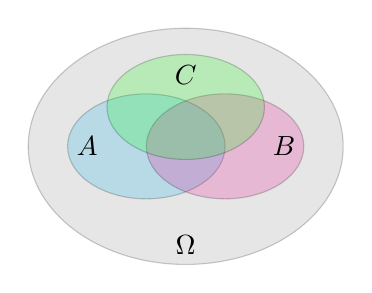
\begin{tikzpicture}[scale = 4/8]
					\draw[fill = gray, opacity=.2] (1,0) ellipse (4 and 3);
					\draw[fill = cyan,opacity = .2](0,0) ellipse (2 and 4/3);
					\draw[fill = magenta,opacity = .2](2,0) ellipse (2 and 4/3);
					\draw[fill = green,opacity = .2](1,1) ellipse (2 and 4/3);
					\draw (-1.5,0) node{$A$};
					\draw (3.5,0) node{$B$};
					\draw (1,1.8) node{$C$};
					\draw(1,-2.5) node {$\Omega$};
				\end{tikzpicture}
			\end{center}
			\item	$\overline{B}\cup C$
			\begin{center}
				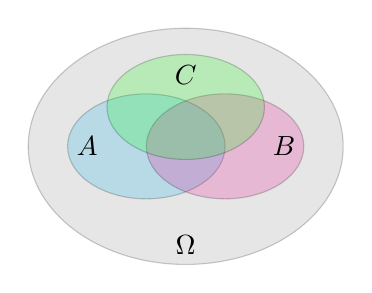
\begin{tikzpicture}[scale = 4/8]
					\draw[fill = gray, opacity=.2] (1,0) ellipse (4 and 3);
					\draw[fill = cyan,opacity = .2](0,0) ellipse (2 and 4/3);
					\draw[fill = magenta,opacity = .2](2,0) ellipse (2 and 4/3);
					\draw[fill = green,opacity = .2](1,1) ellipse (2 and 4/3);
					\draw (-1.5,0) node{$A$};
					\draw (3.5,0) node{$B$};
					\draw (1,1.8) node{$C$};
					\draw(1,-2.5) node {$\Omega$};
				\end{tikzpicture}
			\end{center}
			\item	$\overline{B}\cup \overline{C}$\begin{center}
				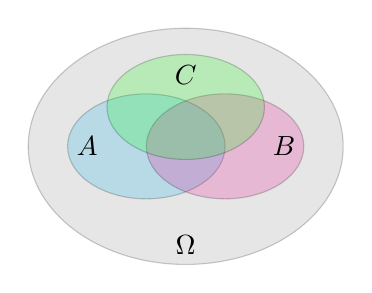
\begin{tikzpicture}[scale = 4/8]
					\draw[fill = gray, opacity=.2] (1,0) ellipse (4 and 3);
					\draw[fill = cyan,opacity = .2](0,0) ellipse (2 and 4/3);
					\draw[fill = magenta,opacity = .2](2,0) ellipse (2 and 4/3);
					\draw[fill = green,opacity = .2](1,1) ellipse (2 and 4/3);
					\draw (-1.5,0) node{$A$};
					\draw (3.5,0) node{$B$};
					\draw (1,1.8) node{$C$};
					\draw(1,-2.5) node {$\Omega$};
				\end{tikzpicture}
			\end{center}
			\item	$\overline{B}\cap \overline{C}$
			\begin{center}
				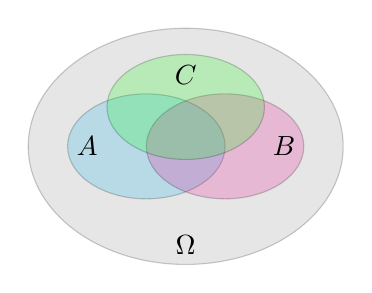
\begin{tikzpicture}[scale = 4/8]
					\draw[fill = gray, opacity=.2] (1,0) ellipse (4 and 3);
					\draw[fill = cyan,opacity = .2](0,0) ellipse (2 and 4/3);
					\draw[fill = magenta,opacity = .2](2,0) ellipse (2 and 4/3);
					\draw[fill = green,opacity = .2](1,1) ellipse (2 and 4/3);
					\draw (-1.5,0) node{$A$};
					\draw (3.5,0) node{$B$};
					\draw (1,1.8) node{$C$};
					\draw(1,-2.5) node {$\Omega$};
				\end{tikzpicture}
			\end{center}
			%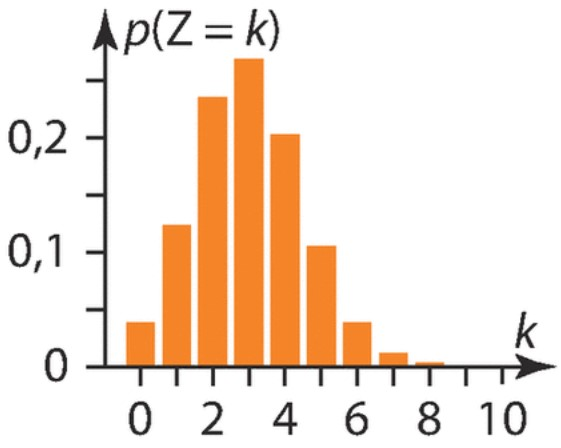
\includegraphics[width=4cm]{diagramme1}
		\end{enumerate}
	\end{multicols}



\exo{ Calculer des probabilités}
On considère deux événements $A$ et $B$.\\
On a : $\ P(A)=0,75\ ;\quad P(B)=0,2\quad$et$\quad P(A\cap B)=0,1$.\\

\dleft{10cm}{
%\begin{multicols}{2}
	\begin{enumerate}
		\item 	Compléter le diagramme de Venn ci-contre :
		%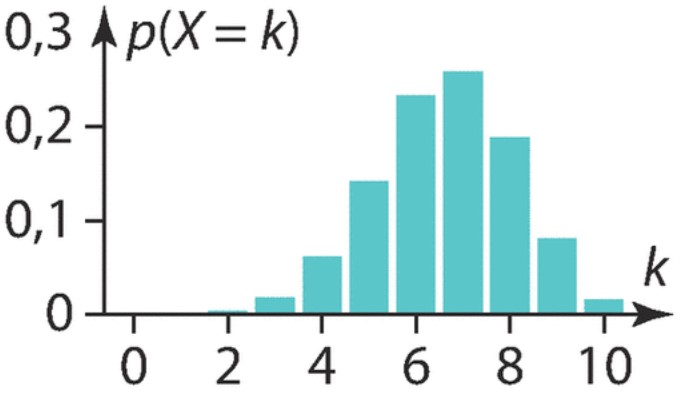
\includegraphics[width=6cm]{diagramme2}
		\item 	Calculer $P(\overline{A})$.
		%\carreauxseyes{7.2}{2.4}
		\item	Compléter l'égalité : \\
		$P(A\cup B)=P(A)+ P(B)$\dotfill
		\item	Calculer $P(A\cup B)$.
		%\carreauxseyes{7.2}{2.4}
		\item	Calculer $P(\overline{A}\cap B)$.
		%\carreauxseyes{7.2}{2.4}
	\end{enumerate}
}
{
    %\begin{center}
        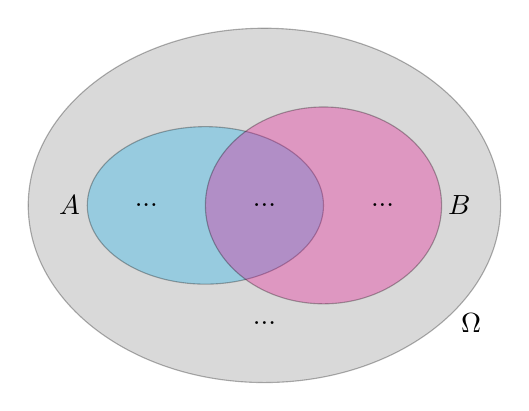
\begin{tikzpicture}[scale = 6/8]
            \draw[fill = gray, opacity=.3] (1,0) ellipse (4 and 3);
            \draw[fill = cyan,opacity = .3](0,0) ellipse (2 and 4/3);
            \draw[fill = magenta,opacity = .3](2,0) ellipse (2 and 5/3);
            \draw (-2.3,0) node{$A$};
            \draw (4.3,0) node{$B$};
            \draw(4.5,-2) node {$\Omega$};
            \draw (-1,0) node{...};
            \draw (3,0) node{...};
            \draw (1,0) node{...};
            \draw(1,-2) node {...};
        \end{tikzpicture}
    %\end{center}
}    
%\end{multicols}

\newpage

\exo{ Utiliser un arbre de dénombrement}
Dans une urne, il y a deux boules rouges $R_1$ et $R_2$ et deux boules noires $N_1$ et $N_2$. On tire deux boules successivement avec remise.
\begin{enumerate}
	\item 	Représenter cette situation par un arbre de dénombrement.
	\item 	Combien y-a-t-il d'issues si on ne considère que la couleur des boules tirées ?
	\item	Quelle est la probabilité des événements suivants :
	\begin{enumalph}
		\item 	A : « obtenir deux boules noires ».
		\item 	B : « obtenir deux boules de la même couleur ».
		\item	C : « obtenir une et une seule boule rouge ».
	\end{enumalph}
\end{enumerate}


\exo{ Utiliser une situation d'équiprobabilité}
On lance un dé équilibré à 20 faces. Les faces sont numérotées de 1 à 20.
\begin{enumerate}
	\item 	Quelle conclusion peut-on tirer du fait que le dé soit équilibré ?
	\item 	Quelle est la probabilité des événements suivants ?
	\begin{enumalph}
		\item 	$A$ : « obtenir un résultat supérieur ou égal à 7 ».
		\item 	$B$ : « obtenir un résultat pair ».
		\item	$C$ : « obtenir un nombre premier ».
		\item	$D=C\cap \overline{B}$.
	\end{enumalph}
\end{enumerate}


\exo{}
On lance un dé truqué à six faces numérotées de 1 à 6 et on observe le résultat obtenu. La loi de probabilité liée à cette expérience aléatoire est donnée ci-dessous avec $x$ et $y$ des réels compris entre 0 et 1.
\begin{center}
	\begin{tabular}{|l|p{1cm}|p{1cm}|p{1cm}|p{1cm}|p{1cm}|p{1cm}|}
		\hline
		\cellcolor{UGLiOrange}Face & \makebox[\linewidth][c]{1} & \makebox[\linewidth][c]{2} & \makebox[\linewidth][c]{3} & \makebox[\linewidth][c]{4} & \makebox[\linewidth][c]{5} & \makebox[\linewidth][c]{6}\\
		\hline
		\cellcolor{UGLiOrange}Probabilité & \makebox[\linewidth][c]{0,1} & \makebox[\linewidth][c]{0,35} & \makebox[\linewidth][c]{0,05} & \makebox[\linewidth][c]{0,2} & \makebox[\linewidth][c]{$x$} & \makebox[\linewidth][c]{$y$}\\
		\hline
	\end{tabular}
\end{center}


On sait de plus que la probabilité d'obtenir un résultat pair est 0,65.
\begin{enumerate}
	\item 	Quelle est la probabilité d'obtenir 6 ?
	\item 	En déduire la probabilité d'obtenir 5.
	\item	Jack affirme que, bien que le dé ne soit pas équilibré, la probabilité d'obtenir un nombre supérieur ou égal à 4 est $\dfrac{1}{2}$. A-t-il raison ?
	\item	Mary affirme de même que la probabilité d'obtenir un nombre premier est aussi $\dfrac{1}{2}$. A-t-elle raison ?
\end{enumerate}


\subsection*{ Probabilités conditionnelles}

\exo{ Détermination de probabilités conditionnelles}

Un artisan produit du miel et de la confiture, de manière industrielle et aussi biologique.\\
Sa production mensuelle est de 900 pots, comprenant notamment :
\begin{enumerate}[label=\textbullet]
	\item 	603 pots de miel, dont 333 sont de fabrication industrielle 
	\item 	63 pots de confiture de fabrication biologique.
\end{enumerate}
\begin{enumerate}
	\item 	Compléter le tableau ci-dessous.
	\begin{center}
		\begin{tabular}{|l|l|l|l|}
			\cline{2-4}
			\multicolumn{1}{l|}{} & Pots de miel & Pots de confiture & \textbf{Total} \\ 
			\hline
			Prod. industrielle &  &  &  \\ 
			\hline
			Prod. Biologique &  &  &  \\ 
			\hline
			\textbf{Total} &  &  &  \textbf{900}\\ 
			\hline
		\end{tabular}\\
	\end{center}
	\item	On choisit au hasard l'un de ces pots.\\
	On considère les évènements suivants :
	\begin{enumerate}[label=\textbullet]
		\item 	C : « c'est un pot de confiture ».
		\item 	B : « c'est un pot de fabrication biologique ».
	\end{enumerate} 
	\begin{enumalph}
		\item 	Calculer les probabilités des évènements B et C et les exprimer en pourcentage.
		\item 	Décrire par une phrase les évènements suivants puis calculer leur probabilité : $\overline{B}$ et $B\cap C$. Exprimer en pourcentage.
		\item	On choisit au hasard un pot parmi les pots de confiture. Quelle est la probabilité qu'il soit de fabrication biologique ? Exprimer à l'aide d'une fraction irréductible. 
		\item 	On choisit au hasard un pot parmi les pots de fabrication biologique. Quelle est la probabilité qu'il s'agisse d'un pot de confiture ? Exprimer à l'aide d'une fraction irréductible.\\
	\end{enumalph}
\end{enumerate} 

\newpage
\exo{ Détermination de probabilités conditionnelles}

Voici les résultats d'un sondage effectué en 1999 auprès de 2\,000 personnes, à propos d'Internet : 
\begin{itemize}
	\item 40\% des personnes interrogées déclarent être intéressées par Internet, 
	\item 35\% des personnes interrogées ont moins de 30 ans et, parmi celles-ci, quatre cinquièmes déclarent être intéressées par Internet, 
	\item 30\% des personnes interrogées ont plus de 60 ans et, parmi celles-ci, 85\% ne sont pas intéressées par Internet. 
\end{itemize} 
\begin{enumerate}
	\item Compléter le tableau suivant :
	\begin{center}
		\begin{tabular}{|c|c|c|c|}
			\hline 
			& intéressées par Internet & non intéressées par internet & \textbf{total} \\
			\hline 
			moins de 30 ans & & & \\
			\hline 
			de 30 à 60 ans & & & \\
			\hline 
			plus de 60 ans & & & \\
			\hline 
			\textbf{total} & & & \textbf{2\,000} \\
			\hline 
		\end{tabular} 
	\end{center}
	\item On choisit au hasard une personne parmi les 2\,000 interrogées. On suppose que toutes les personnes ont la même probabilité d'être choisies. On considère les événements :
	\begin{itemize} 
		\item[A :]« {\sl la personne interrogée a moins de 30 ans}»
		\item[B :] « {\sl la personne interrogée est intéressée par Internet}»
	\end{itemize}
	\begin{enumalph}
		\item Calculer les probabilités $P(A)$ et $P(B)$. 
		\item Définir par une phrase l'événement $A\cap B$ puis calculer $P(A\cap B)$.
	\end{enumalph}
	\item On sait maintenant que la personne interrogée est intéressée par Internet.\\               
	Quelle est la probabilité qu'elle ait plus de 30 ans ? Comment note-t-on cette probabilité ?
	\item Calculer $P_{\overline{A}}(B)$ et interpréter cette probabilité conditionnelle.\\
\end{enumerate} 

\exo{ Avec un arbre}
\dleft{10.5cm}{
	On considère deux événements $A$ et $B$ dont les probabilités sont données par l'arbre ci-contre :
	\begin{enumerate}
		\item 	Compléter cet arbre pondéré.
		\item 	Quelle est la probabilité que $B$ se réalise sachant que $A$ n'est pas réalisé ?\\
	\end{enumerate}
}{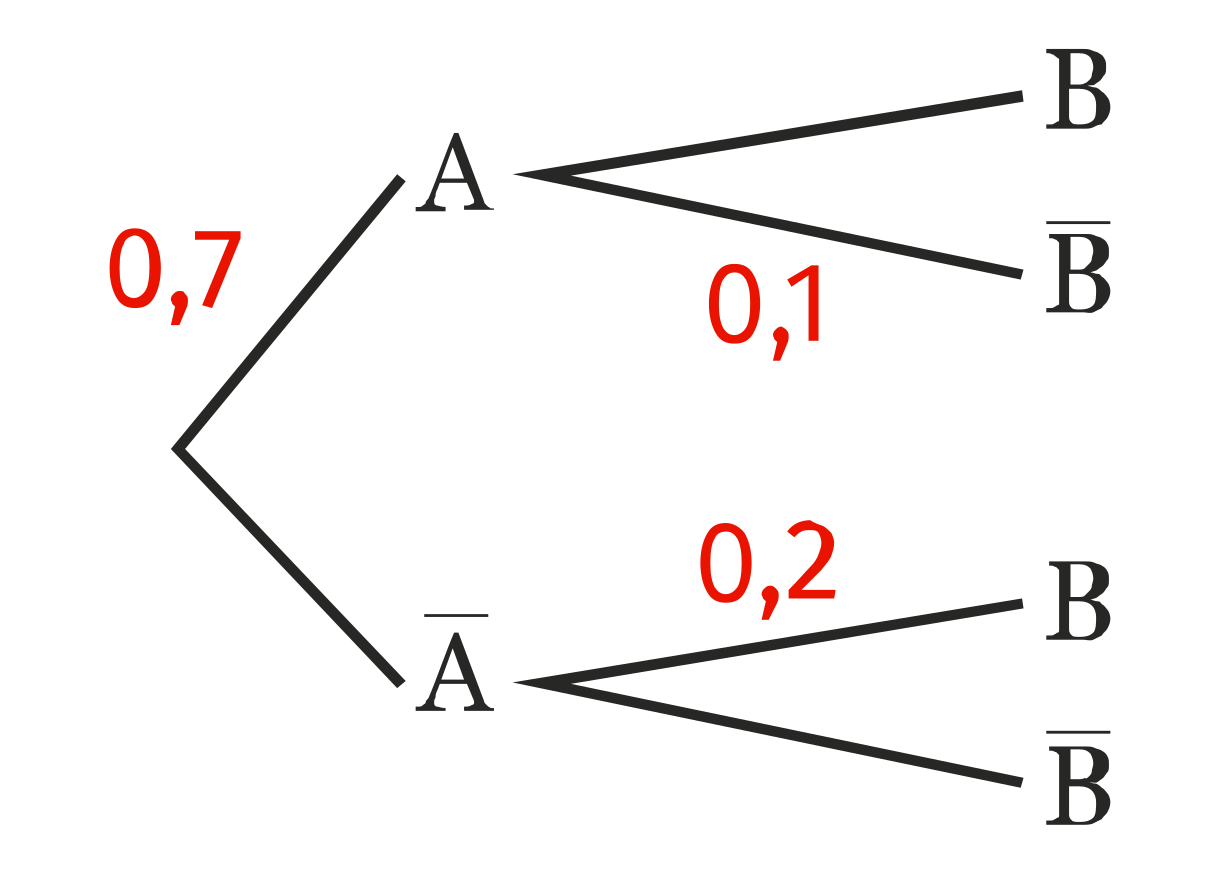
\includegraphics[width=4.5cm]{arbre}}


%\newpage
\exo{}

On choisit au hasard une figure parmi les suivantes. Chaque figure a la même probabilité d'être choisie.
\begin{center}
	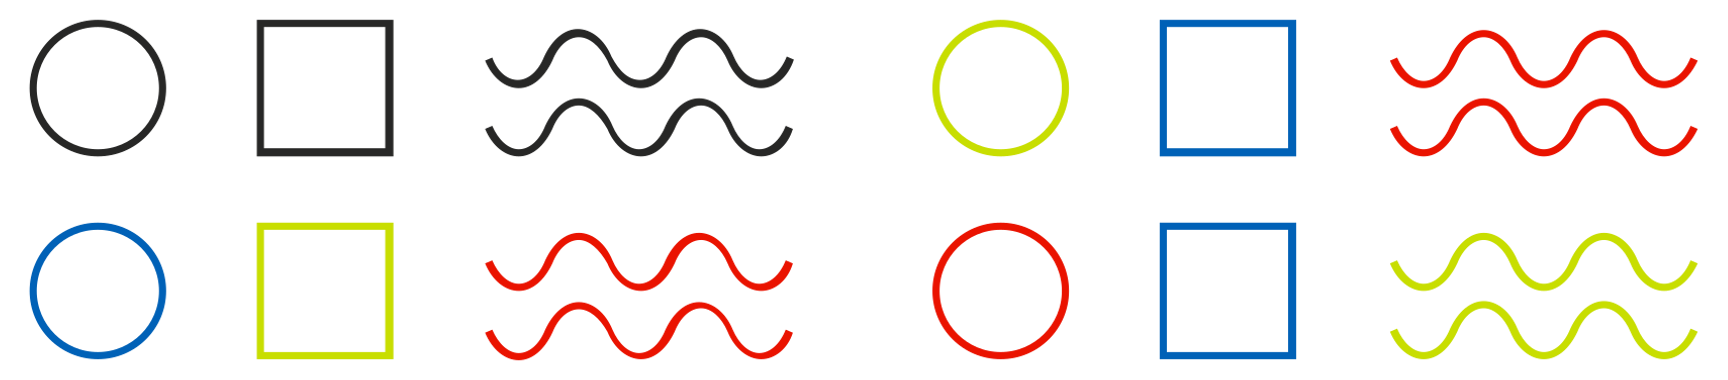
\includegraphics[width=12cm]{figures}
\end{center}
On considère les événements suivants :
\begin{enumerate}[label=\textbullet]
	\item 	$V$ : « la figure est verte » ;
	\item 	$R$ : « la figure est rouge » ;
	\item 	$N$ : « la figure est noire » ;
	\item 	$B$ : « la figure est bleue » ;
	\item 	$C$ : « la figure est un cercle » ;
	\item 	$K$ : « la figure est un carré » ;
	\item	$Z$ : « la figure fait des vagues ».
\end{enumerate}
\begin{enumerate}
	\item 	Modéliser cette situation par un tableau.
	\item 	Calculer $P_C(V)$ et $P_B(Z)$.
	\item	Calculer $P_R(Z)$ et $P_K(B)$.
\end{enumerate}

\exo{}

Dans une forêt, il y a 30 \% d'épicéas et 70 \% de sapins. 10 \% des arbres ont un parasite. Les épicéas représentent 20 \% des arbres touchés.\\

Quelle est la probabilité qu'un épicéa soit touché par le parasite ?\\


\exo{ Utilisation des probabilités conditionnelles}

Dans un restaurant d'entreprise, on propose 2 formules : la A et la B. On remarque que chaque client choisit le menu A avec une probabilité de 40\%.
Sinon, la probabilité que le client ne prenne pas de café est de 55\%.\\

Quelle est la probabilité qu'un client choisisse le menu B et un café ?\\


\end{document}


